% !TeX root = RJwrapper.tex
\title{animbook: Visualizing changes in performance measures and demographic affiliations using animation}


\author{by Krisanat Anukarnsakulchularp}

\maketitle

\abstract{%
An abstract of less than 150 words.
}

\hypertarget{introduction}{%
\section{Introduction}\label{introduction}}

The concept of ``zombie companies'' began to attract attention when an article on the proliferation of zombie companies (Caballero, Hoshi, and Kashyap (2008)). The ``zombie companies'' are generally defined as companies with an interest coverage ratio of less than one for a period of more than three years. However, there is a simpler and more easily understandable way to show these concepts by visualizing the new listings (enters) and the de-listing (exits) of publicly traded companies on a country-by-country basis. This visualization method makes it clear that the concepts of zombie companies are not unique to Japan, as indicated in the OECD report (McGowan, Andrews, and Millot (2017)) that the United States has a faster metabolize (more new listings and exits) relative to Japan.

The visualization above can also be thought of as a movement between groups, which is how many companies have entered the market and how many have exited the market. One example of this visualization is from The New York Times article ``Extensive data shows punishing reach of racism for black boys'' (Badger et al. (2018)). The animation portrays the trajectory of how boys with different demographics could land up in society. It can be adapted to our problems by capturing the movement between the groups over a specific period.

With an advancement in technology, this results in an increase in both the size and complexity of the data. It requires an experienced hand to convey the right messages from the data. However, as shown in The New York Times article (Badger et al. (2018)), the animation is not only created just for eye-catching graphics. Animation can be used as a tool that helps communicate complex data, enhancing the narrative and keeping it engaged for the audience. Based on Mayer and Moreno (2002), animation can improve learning, especially when the goal is to promote deep understanding. It also requires the designer to understand how people learn. The cognitive theory of multimedia learning (Mayer (2005)) will be considered during the designing period.

The challenge of the New York Times article animation was the amount of code needed to reproduce. Additionally, the business data may or may not have the same information as the one in the article. These two purposes establish the objective for creating the R package that could generalize the animation to a wider range of data.

The structure of this paper will consist of both the visualization design and software design. The first section will explain about the animation in The New York Times article. Secondly, what are the expected data to be input into the plot, and how it is processed. The third section is about the animation tools, for example, \textbf{gganimate} (Pedersen and Robinson (2020)) and \textbf{plotly} (Sievert (2020)). The next section will be about the design of the package and visualization. The last two sections explore the usage of the R package and the application.

\hypertarget{explanation-of-the-new-york-times-visualization}{%
\section{Explanation of the New York Times visualization}\label{explanation-of-the-new-york-times-visualization}}

The flow chart featured in one of the New York Time articles unveils the issue of income disparities between black and white children who were raised in families with comparable income according to the Chetty et al. (2020). This visualization reveals that, compared to white children, black children are more likely to drop down to the lower-income group, given that they both grew up in wealthy families.

In the visualization, each observation is initially classified into one group at the start and potentially transitions into either the same group or a different group. This dynamics visualization constructs questions on the broader use of this visualization to other types of data. As mentioned in the introduction, one of the data that will make use of this is accounting data. Additionally, the marketing data that exhibits the movement of customers shifting the product interest to another competitor can be valuable insight into the data. It could be extended to incorporate demographic information of the customers. It would allow the marketing analyst to gain a significant understanding of both the company's products and the overall market. This also applies to the election data for the analyst to consolidate the campaign for their political party.

This animation was developed using two software based on JavaScript, D3.js (Bostock (2012)), and WebGL (reference). The D3 JavaScript is one of the most widely known libraries for creating an interactive and dynamic visualization. It enables the designers to bind both the data and graphical elements to the DOM (Document Object Model). On the other hand, WebGL functions as a JavaScript API for rendering interactive 2D and 3D graphics within any compatible web browser without the use of plug-ins. For the animation in this paper, the programming languages that will be used for recreating and revising the visualization done by The New York Times articles is R (R Core Team (2021)).

\hypertarget{data}{%
\section{Data}\label{data}}

Before any visualizations can be performed, the users must first understand the data concept known as \texttt{tidy\ data} (Wickham (2014)). There are three fundamental key principles: each variable forms a column, each observation forms a row, and each type of observational unit forms a table. These three keys are Codd's third normal form (Codd (1990)), but phrase in the language of statistics. The tidy data format focuses on a single dataset instead of many connected datasets typically found in a relational database.

The accounting data that will be used in this section and in most of the examples for this paper was collected from Bureau van Dijk (reference). This data set comprises 30,000 rows and 94 variables of information on listed and major unlisted/delisted companies worldwide. The only variables of interest from this data set are ID, year, country, and sales. A subset version of this data set, which only contained variables of interest from 2006 to 2018, is included in this package.

Now that the tidy data concept is established and the example data is introduced, let's explore how the data got transformed. As seen in the visualization, each observation is classified into a group. In the accounting data, however, it is represented in a numerical form instead of categories. The numerical value needs to be somehow mapped to a category. One way to handle this is by ranking the sales and grouping the rankings into quantiles. In some cases, this may not be the best option. As the observation is moved up by quantiles, one is bound to move down. It can be resolved by using an alternative method, which is grouping values based on their absolute values. Users may also be interested in grouping the data based on different demographics, for example, ranking within a specific country. This generalization leads to a total of four scaling methods for the numerical data.

Original data:

\begin{verbatim}
#> # A tibble: 12 x 4
#>    ID           year    sales country
#>    <fct>       <int>    <dbl> <fct>  
#>  1 AU004085330  2007  1043282 AU     
#>  2 AU004085330  2006   846245 AU     
#>  3 AU009134114  2006    67842 AU     
#>  4 AU009134114  2007    47868 AU     
#>  5 AU009219809  2007   326335 AU     
#>  6 AU009219809  2006   218384 AU     
#>  7 US161229730  2007     5991 US     
#>  8 US161229730  2006     4308 US     
#>  9 US470731996  2007  8126500 US     
#> 10 US470731996  2006  7205000 US     
#> 11 US751825172  2007 22935000 US     
#> 12 US751825172  2006 22563000 US
\end{verbatim}

\begin{enumerate}
\def\labelenumi{\arabic{enumi}.}
\tightlist
\item
  Ranking by year.
\end{enumerate}

\begin{verbatim}
#> # A tibble: 12 x 4
#>    id           time qtile country
#>    <fct>       <int> <dbl> <fct>  
#>  1 AU004085330  2006     2 AU     
#>  2 AU004085330  2007     2 AU     
#>  3 AU009134114  2006     3 AU     
#>  4 AU009134114  2007     3 AU     
#>  5 AU009219809  2006     3 AU     
#>  6 AU009219809  2007     2 AU     
#>  7 US161229730  2006     4 US     
#>  8 US161229730  2007     4 US     
#>  9 US470731996  2006     1 US     
#> 10 US470731996  2007     1 US     
#> 11 US751825172  2006     1 US     
#> 12 US751825172  2007     1 US
\end{verbatim}

\begin{enumerate}
\def\labelenumi{\arabic{enumi}.}
\setcounter{enumi}{1}
\tightlist
\item
  Fix bins relative to absolute values by year.
\end{enumerate}

\begin{verbatim}
#> # A tibble: 12 x 4
#>    id           time qtile country
#>    <fct>       <int> <dbl> <fct>  
#>  1 AU004085330  2006     5 AU     
#>  2 AU004085330  2007     5 AU     
#>  3 AU009134114  2006     5 AU     
#>  4 AU009134114  2007     5 AU     
#>  5 AU009219809  2006     5 AU     
#>  6 AU009219809  2007     5 AU     
#>  7 US161229730  2006     5 US     
#>  8 US161229730  2007     5 US     
#>  9 US470731996  2006     4 US     
#> 10 US470731996  2007     4 US     
#> 11 US751825172  2006     1 US     
#> 12 US751825172  2007     1 US
\end{verbatim}

\begin{enumerate}
\def\labelenumi{\arabic{enumi}.}
\setcounter{enumi}{2}
\tightlist
\item
  Ranking by year within a group.
\end{enumerate}

\begin{verbatim}
#> # A tibble: 12 x 4
#>    id           time qtile country
#>    <fct>       <int> <dbl> <fct>  
#>  1 AU004085330  2006     4 AU     
#>  2 AU004085330  2007     4 AU     
#>  3 AU009134114  2006     4 AU     
#>  4 AU009134114  2007     4 AU     
#>  5 AU009219809  2006     4 AU     
#>  6 AU009219809  2007     4 AU     
#>  7 US161229730  2006     4 US     
#>  8 US161229730  2007     3 US     
#>  9 US470731996  2006     1 US     
#> 10 US470731996  2007     1 US     
#> 11 US751825172  2006     1 US     
#> 12 US751825172  2007     1 US
\end{verbatim}

\begin{enumerate}
\def\labelenumi{\arabic{enumi}.}
\setcounter{enumi}{3}
\tightlist
\item
  Fix bins relative to absolute values by year within a group (bug in code).
\end{enumerate}

\begin{verbatim}
#> # A tibble: 12 x 4
#>    id           time qtile country
#>    <fct>       <int> <dbl> <fct>  
#>  1 AU004085330  2006     5 AU     
#>  2 AU004085330  2007     5 AU     
#>  3 AU009134114  2006     5 AU     
#>  4 AU009134114  2007     5 AU     
#>  5 AU009219809  2006     5 AU     
#>  6 AU009219809  2007     5 AU     
#>  7 US161229730  2006     5 US     
#>  8 US161229730  2007     5 US     
#>  9 US470731996  2006     4 US     
#> 10 US470731996  2007     4 US     
#> 11 US751825172  2006     1 US     
#> 12 US751825172  2007     1 US
\end{verbatim}

For the first and third scaling methods, group splitting is executed using the \texttt{quantiles()} and \texttt{cut()} functions. The \texttt{quantile} function from the \texttt{stats} R package (R Core Team (2013)) takes a numeric vector and outputs the corresponding quantiles to the given probabilities. The output from the \texttt{quantile} function is then used as the \texttt{breaks} argument for the cut function that is part of the base R packages.

In contrast, the second and fourth scaling methods calculate the quantile based on the absolute values scales. The default approach is to break the group equally using the \texttt{seq()} function. The \texttt{seq()} function takes input values from the minimum and maximum values and increments by equal steps depending on the number of groups of interest.

\begin{figure}

{\centering 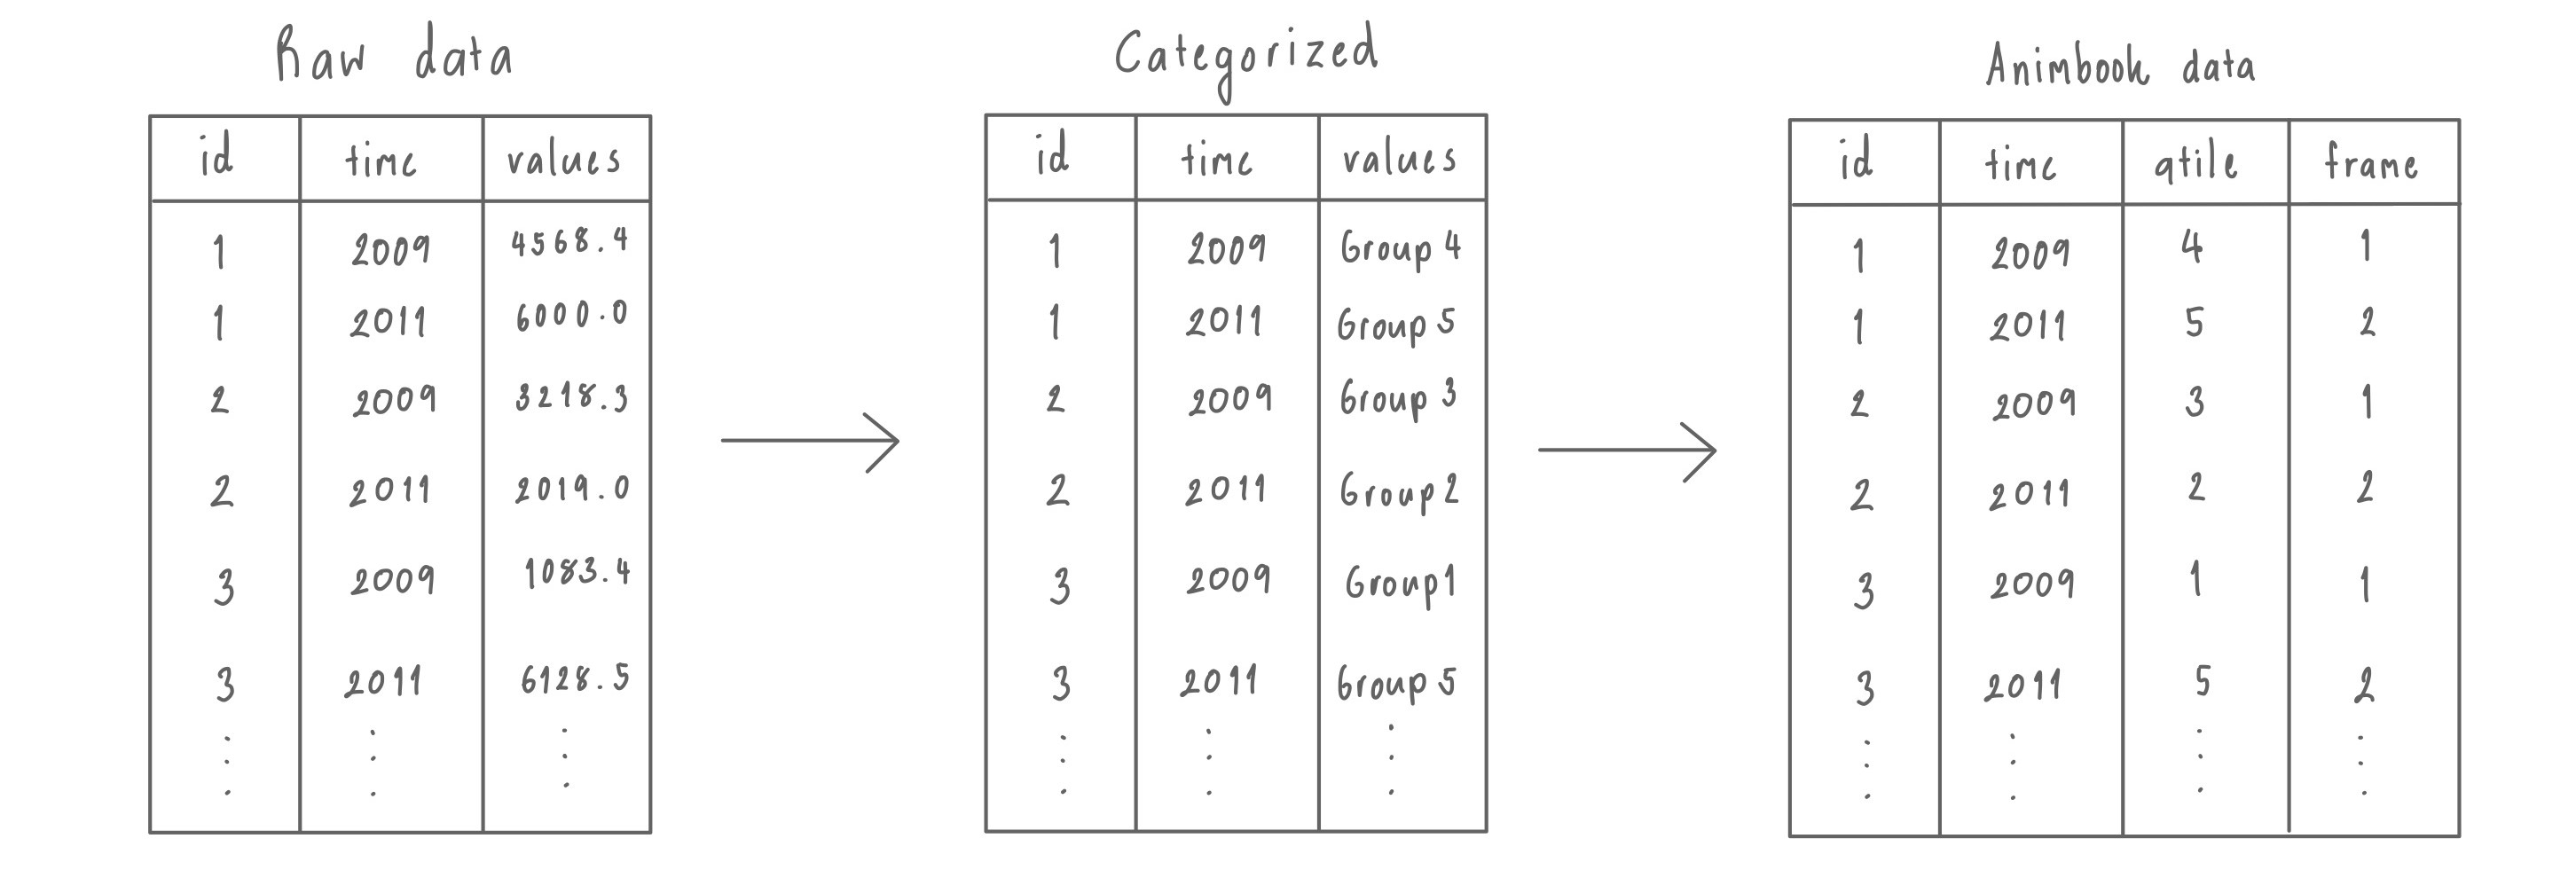
\includegraphics[width=1\linewidth]{figures/data-diagram} 

}

\caption{The data transformation diagram.}\label{fig:data-diagram}
\end{figure}

Based on Figure \ref{fig:data-diagram}, these are only the initial steps in formatting the data into a category. Now that there is a method to transform the data from the raw into a categorized format, the next step is to modify it into an animbook data structure. It is carried out by assigning the frame to each individual observation, ensuring that each ID does not contain repeat frame values. Its lets the \textbf{gganimate} or \textbf{plotly} to perceive where the observation would be on the plot at a given frame.

The frame variable is assigned by sorting the data based on the id and time using the \texttt{arrange()} function, followed by applying the \texttt{group\_by()} function on the id, allowing the \texttt{row\_number()} function to be performed within each group. The functions mentioned in this paragraph are from the \texttt{dplyr} packages (Wickham et al. (2023)).

\hypertarget{animation-tools}{%
\section{Animation tools}\label{animation-tools}}

Literature review of animation tools

\hypertarget{visualization-design}{%
\section{Visualization design}\label{visualization-design}}

This explains how to get from data to the animations, including different sorts of plots.

\hypertarget{software}{%
\section{Software}\label{software}}

\hypertarget{installation}{%
\subsection{Installation}\label{installation}}

\hypertarget{overview-of-functions}{%
\subsection{Overview of functions}\label{overview-of-functions}}

In designing the package for reproducing the New York Times animated plot, the package ended up with a three-step process in recreating the animation. The first step is to turn the data into the right format for the plot function. The next stage is to create a ggplot object, which can then be inputted into the animation function. The last step is adding the animation settings to the ggplot object so the user can animate the plot using the \texttt{gganimate::animate()} function. The reason for this three-step process is that it allows the user who does not have a lot of experience to reproduce the animation while keeping the customization for an experienced user.

\hypertarget{prepare-the-data}{%
\subsubsection{Prepare the data}\label{prepare-the-data}}

The first step can be done using the \texttt{anim\_prep()} function. This function required that the user data contained ID, which is used to identify each individual observation, values, which are numerical values to be used to group the observation together, and time, the variable associated with the changes of the observation. In the cases when the users already have the values as a group variable, the \texttt{anim\_prep\_cat()} function can then be used instead.

The additional options for the \texttt{anim\_prep()} that allow for more customization to the data structure or the plot are as follows:

\begin{itemize}
\tightlist
\item
  label: group labeling.
\item
  ngroup: number of groups we want to split the values into.
\item
  breaks: the group bins' size
\item
  group\_scaling: the grouping variable for the bins calculations.
\item
  color: the variable used to color the observations.
\item
  time\_dependent: logical. Whether we want the observations to start at the same time or not.
\item
  scaling: the scaling method, either \texttt{rank} or \texttt{absolute}.
\item
  runif\_min: minimum value for random addition to frame numbers
\item
  runif\_max: maximum value for random addition to frame numbers
\end{itemize}

Using the different combinations of the additional options, the users could end up with four different scales, as mentioned in the \ref{data} section.

\begin{enumerate}
\def\labelenumi{\arabic{enumi}.}
\item
  Rank scaling
\item
  Absolute scaling
\item
  Rank scaling by group
\item
  Absolute scaling by group
\end{enumerate}

For the \texttt{anim\_prep\_cat()} function, the additional options are:

\begin{itemize}
\tightlist
\item
  label: group labeling.
\item
  order: the ordering of the group.
\item
  color: the variable used to color the observations.
\item
  time\_dependent: logical. Whether we want the observations to start at the same time or not.
\item
  runif\_min: minimum value for random addition to frame numbers
\item
  runif\_max: maximum value for random addition to frame numbers
\end{itemize}

Both the \texttt{anim\_prep()} and \texttt{anim\_prep\_cat()} functions will return the ``animbook'' object containing a list of the standard format data and settings.

\hypertarget{plotting-the-data}{%
\subsubsection{Plotting the data}\label{plotting-the-data}}

Once the data is prepared. The next step is to create the ggplot object as a basis for the animation. There are three plots available in this package. Two of the plots could be used for the animation, and another plot is used as a static visualization.

\begin{itemize}
\tightlist
\item
  \texttt{kangaroo\_plot()}: plots the observation's movement over time.
\item
  \texttt{wallaby\_plot()}: the subset plot of the \texttt{kangaroo\_plot} with the time limit to only start and end.
\item
  \texttt{funnel\_web\_plot()}: the faceted static plot by time variable.
\end{itemize}

All of the plots have an internal function that converts the standard data format into the required structure for each plotting function.

\begin{enumerate}
\def\labelenumi{\arabic{enumi}.}
\tightlist
\item
  Kangaroo's plot
\end{enumerate}

\includegraphics[width=0.7\linewidth]{animbook-journal_files/figure-latex/unnamed-chunk-13-1}

\begin{enumerate}
\def\labelenumi{\arabic{enumi}.}
\setcounter{enumi}{1}
\tightlist
\item
  Wallaby's plot
\end{enumerate}

\includegraphics[width=0.7\linewidth]{animbook-journal_files/figure-latex/unnamed-chunk-14-1}

\begin{enumerate}
\def\labelenumi{\arabic{enumi}.}
\setcounter{enumi}{2}
\tightlist
\item
  Funnel web spider's plot
\end{enumerate}

\includegraphics[width=0.7\linewidth]{animbook-journal_files/figure-latex/unnamed-chunk-15-1}

\hypertarget{animating-the-plot}{%
\subsubsection{Animating the plot}\label{animating-the-plot}}

To animate the plot, the plot need to be save as an object before passed on to the final function \texttt{anim\_animate()}.

\hypertarget{example-usage}{%
\subsection{Example usage}\label{example-usage}}

\hypertarget{application}{%
\section{Application}\label{application}}

\hypertarget{accounting-database-osiris}{%
\subsection{Accounting database: osiris}\label{accounting-database-osiris}}

\hypertarget{voter-behavior}{%
\subsection{Voter behavior}\label{voter-behavior}}

Based on the 2016 Australian election results, how does the top party perform in keeping the old voters for different genders.

\hypertarget{references}{%
\section*{References}\label{references}}
\addcontentsline{toc}{section}{References}

\hypertarget{refs}{}
\begin{CSLReferences}{1}{0}
\leavevmode\vadjust pre{\hypertarget{ref-the_new_york_time}{}}%
Badger, Emily, Claire Cain Miller, Adam Pearce, and Kevin Quealy. 2018. {``Extensive Data Shows Punishing Reach of Racism for Black Boys.''} \emph{The New York Times}. The New York Times. \url{https://www.nytimes.com/interactive/2018/03/19/upshot/race-class-white-and-black-men.html}.

\leavevmode\vadjust pre{\hypertarget{ref-d3js}{}}%
Bostock, Mike. 2012. {``D3.js - Data-Driven Documents.''} 2012. \url{http://d3js.org/}.

\leavevmode\vadjust pre{\hypertarget{ref-zombie_companies_2008}{}}%
Caballero, Ricardo J., Takeo Hoshi, and Anil K. Kashyap. 2008. {``Zombie Lending and Depressed Restructuring in Japan.''} \emph{The American Economic Review} 98 (5): 1943--77. \url{http://www.jstor.org/stable/29730158}.

\leavevmode\vadjust pre{\hypertarget{ref-race}{}}%
Chetty, Raj, Nathaniel Hendren, Maggie Jones, and Sonya Porter. 2020. {``Race and Economic Opportunity in the United States: An Intergenerational Perspective*.''} \emph{The Quarterly Journal of Economics} 135 (May): 711--83. \url{https://doi.org/10.1093/qje/qjz042}.

\leavevmode\vadjust pre{\hypertarget{ref-relational}{}}%
Codd, E. F. 1990. \emph{The Relational Model for Database Management: Version 2}. USA: Addison-Wesley Longman Publishing Co., Inc.

\leavevmode\vadjust pre{\hypertarget{ref-mayer_2005}{}}%
Mayer, Richard E. 2005. {``Cognitive Theory of Multimedia Learning.''} In \emph{The Cambridge Handbook of Multimedia Learning}, edited by RichardEditor Mayer, 31--48. Cambridge Handbooks in Psychology. Cambridge University Press. \url{https://doi.org/10.1017/CBO9780511816819.004}.

\leavevmode\vadjust pre{\hypertarget{ref-Mayer_Moreno_2002}{}}%
Mayer, Richard E., and Roxana Moreno. 2002. \emph{Educational Psychology Review} 14 (1): 87--99. \url{https://doi.org/10.1023/a:1013184611077}.

\leavevmode\vadjust pre{\hypertarget{ref-oecd_report}{}}%
McGowan, Müge Adalet, Dan Andrews, and Valentine Millot. 2017. {``The Walking Dead?''} no. 1372. https://doi.org/\url{https://doi.org/https://doi.org/10.1787/180d80ad-en}.

\leavevmode\vadjust pre{\hypertarget{ref-gganimate}{}}%
Pedersen, Thomas Lin, and David Robinson. 2020. {``Gganimate: A Grammar of Animated Graphics.''} \emph{R Package Version} 1 (7): 403--8.

\leavevmode\vadjust pre{\hypertarget{ref-stats}{}}%
R Core Team. 2013. \emph{R: A Language and Environment for Statistical Computing}. Vienna, Austria: R Foundation for Statistical Computing. \url{http://www.R-project.org/}.

\leavevmode\vadjust pre{\hypertarget{ref-r}{}}%
---------. 2021. \emph{R: A Language and Environment for Statistical Computing}. Vienna, Austria: R Foundation for Statistical Computing. \url{https://www.R-project.org/}.

\leavevmode\vadjust pre{\hypertarget{ref-plotly}{}}%
Sievert, Carson. 2020. {``Interactive {Web-Based} Data Visualization with r, Plotly, and Shiny.''} Chapman; Hall/CRC. \url{https://plotly-r.com}.

\leavevmode\vadjust pre{\hypertarget{ref-tidy-data}{}}%
Wickham, Hadley. 2014. {``Tidy Data.''} \emph{Journal of Statistical Software} 59 (10): 1--23. \url{https://doi.org/10.18637/jss.v059.i10}.

\leavevmode\vadjust pre{\hypertarget{ref-dplyr}{}}%
Wickham, Hadley, Romain François, Lionel Henry, Kirill Müller, and Davis Vaughan. 2023. \emph{Dplyr: A Grammar of Data Manipulation}.

\end{CSLReferences}

\bibliography{animbook-journal.bib}

\address{%
Krisanat Anukarnsakulchularp\\
Monash University\\%
Faculty of Business and Economics\\ Melbourne, Australia\\
%
%
\textit{ORCiD: \href{https://orcid.org/0009-0008-5638-7124}{0009-0008-5638-7124}}\\%
\href{mailto:kanu0003@student.monash.edu}{\nolinkurl{kanu0003@student.monash.edu}}%
}
